\subsection{Prototyping}
\label{subsec:proto}
\begin{figure}[hbtp]
\centering
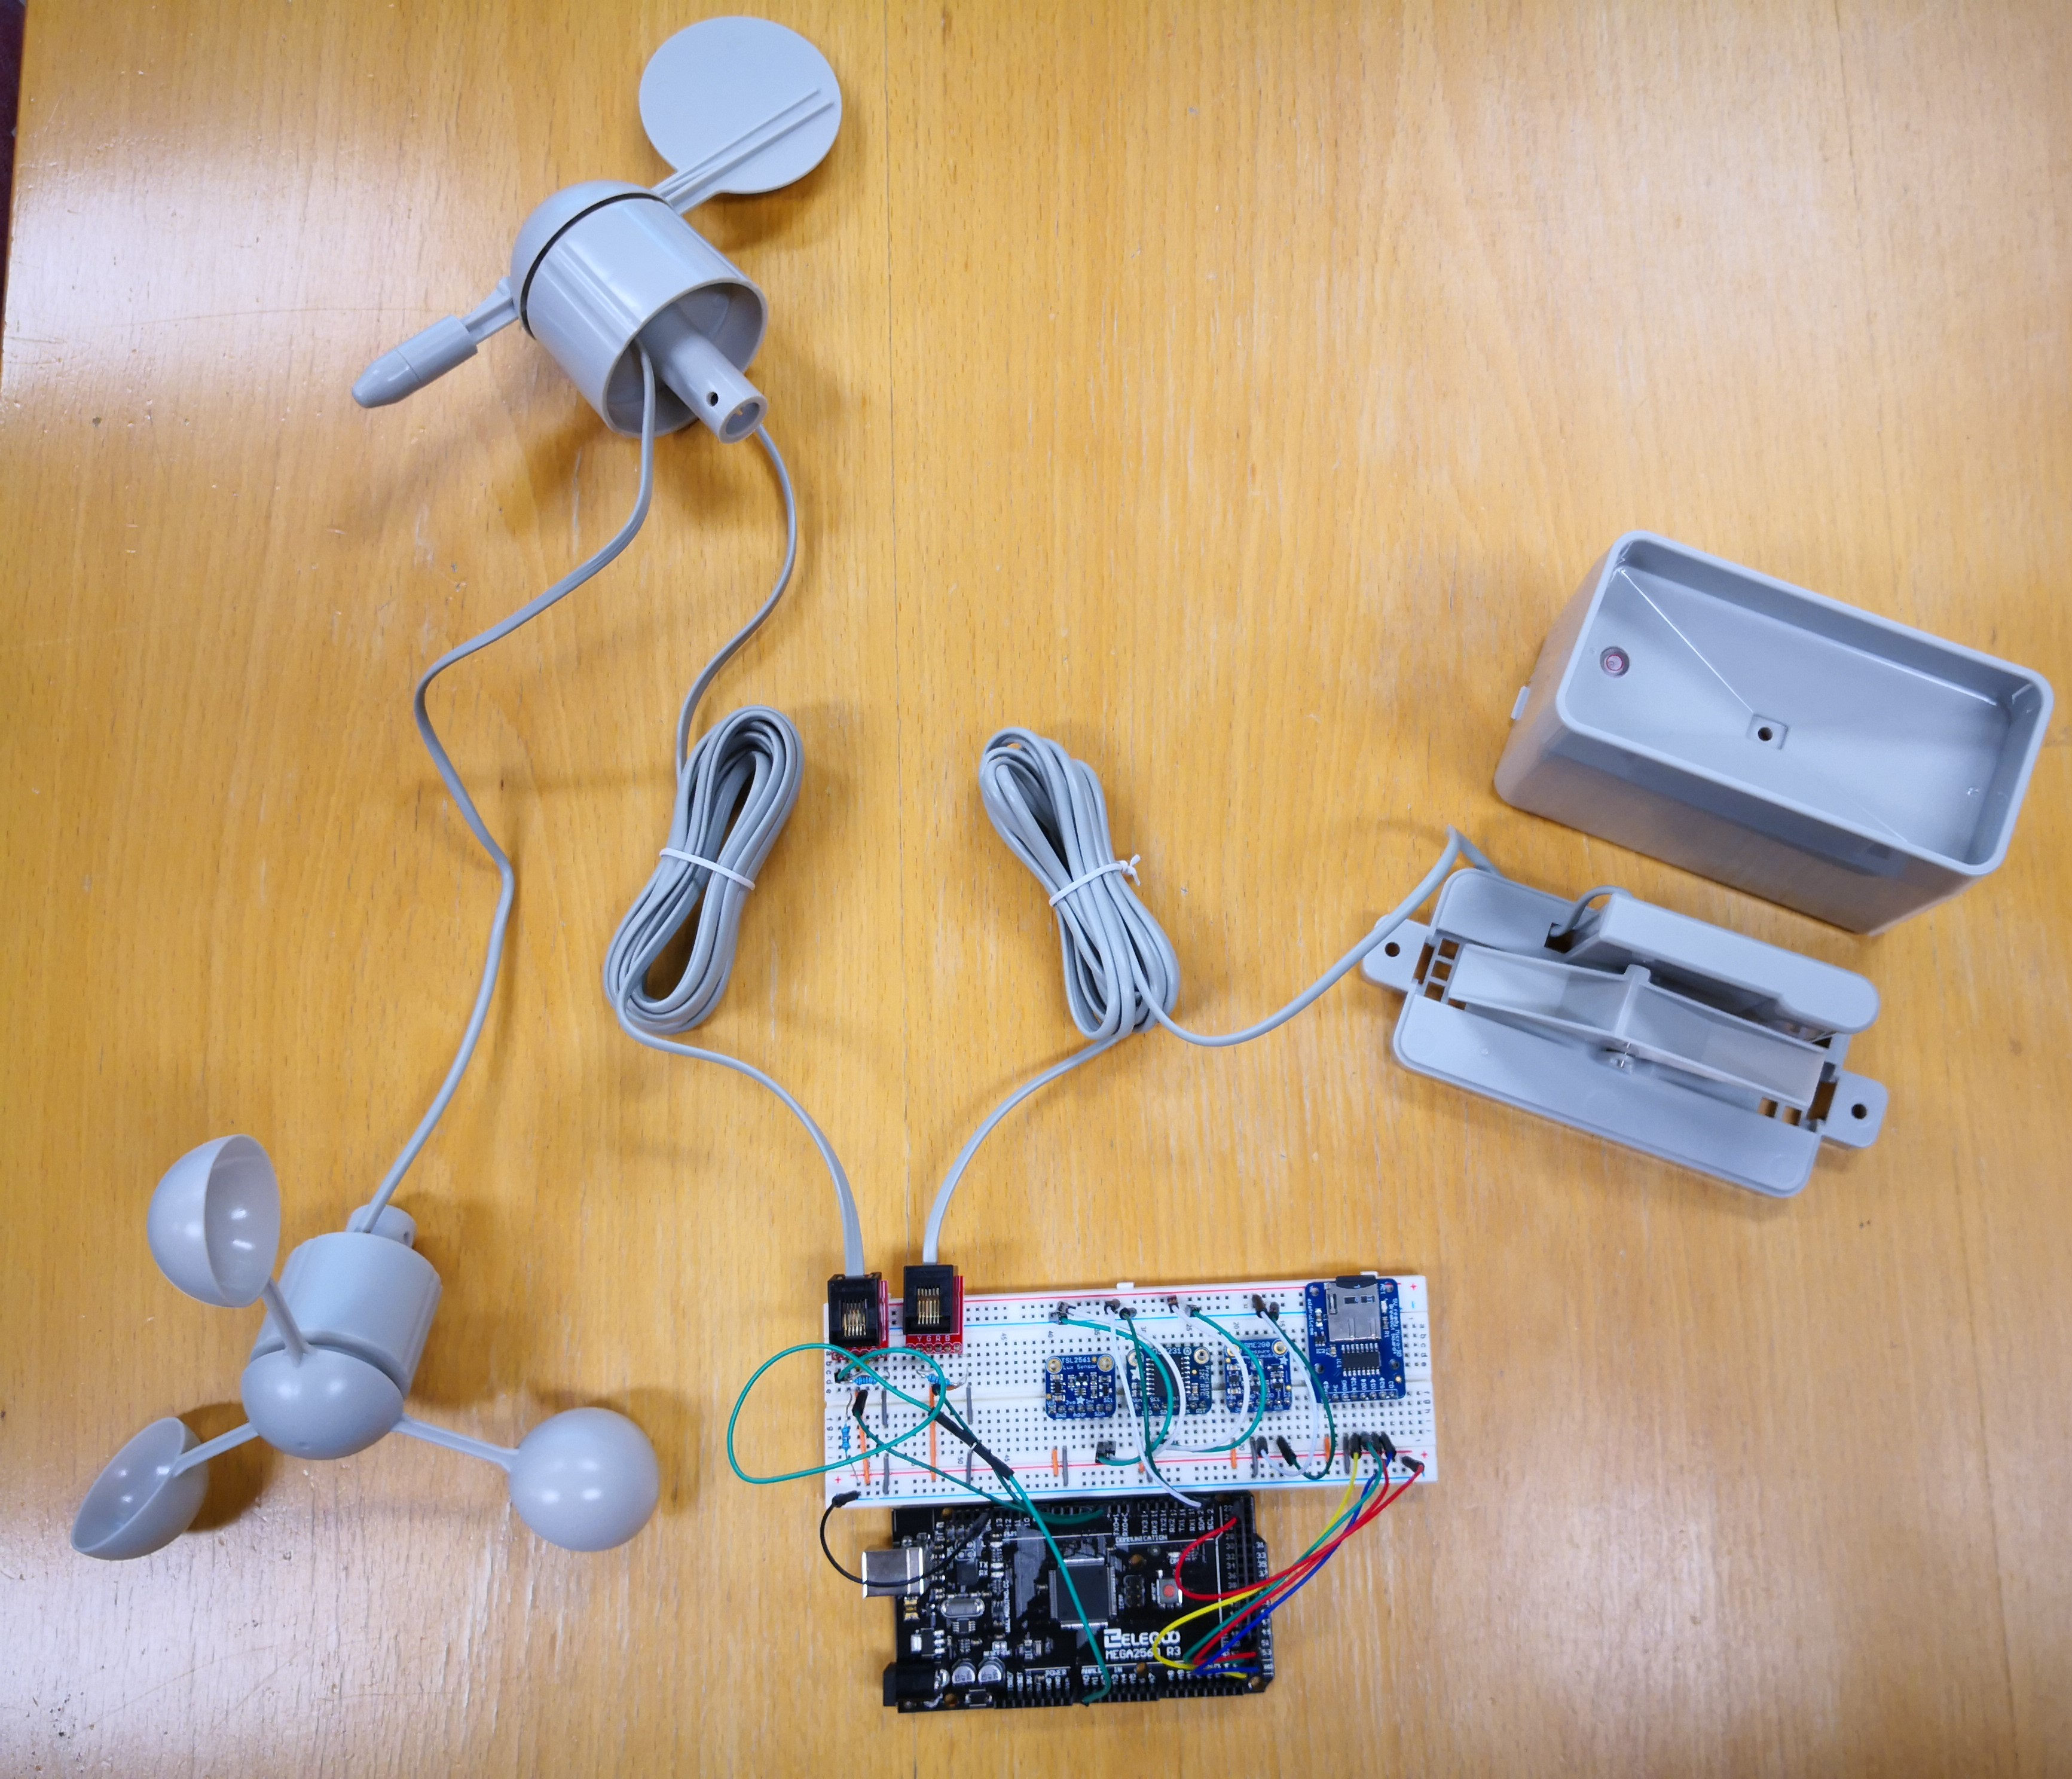
\includegraphics[width=0.9\textwidth]{graphics/prototyping/komplett.jpg} 
\caption{Prototyping mittels Breakoutboards}
\end{figure}

Der erste funktionierende Prototyp wurde auf einem Breadboard realsiert. Für die Implementierung aller partiellen Systemen sind hauptsächlich Breakoutboards von Adafruit mit den entsprechenden Chips verwendet worden.\\

{\begin{minipage}[b][5cm][t]{0.3\textwidth}
\centering
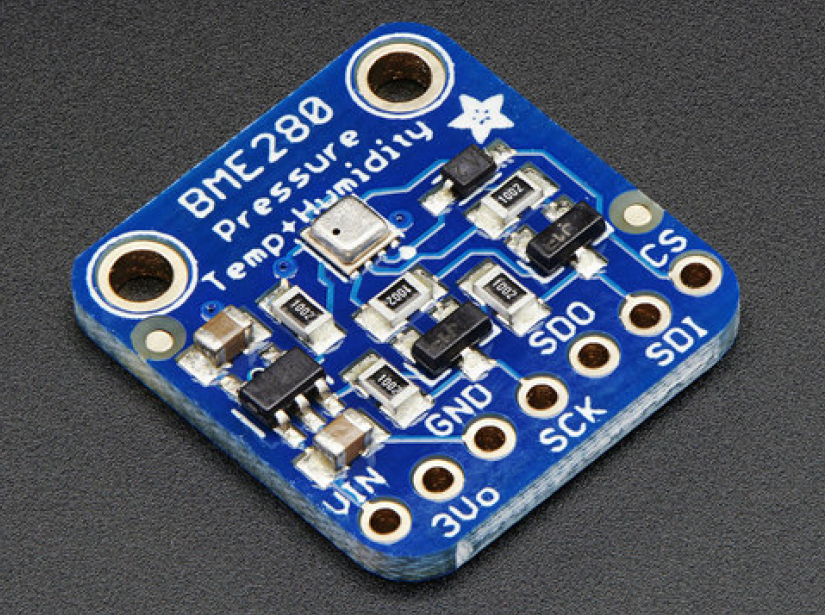
\includegraphics[width=\textwidth]{graphics/prototyping/bme280.PNG} 
\captionof{figure}{BME280 Breakoutboard \cite{LadyAdabme2802018}}
\label{fig:bme280_breakoutboard}
\end{minipage}}
{\begin{minipage}[b][5cm][t]{0.3\textwidth}
\centering
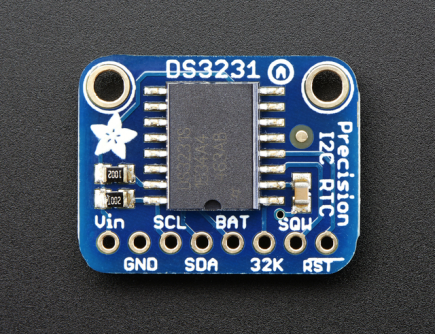
\includegraphics[width=\textwidth]{graphics/prototyping/DS3231.png} 
\captionof{figure}{DS3231 Breakoutboard \cite{LadyAda2018ds3231}}
\label{fig:ds3231_breakoutboard}
\end{minipage}}
{\begin{minipage}[b][5cm][t]{0.3\textwidth}
\centering
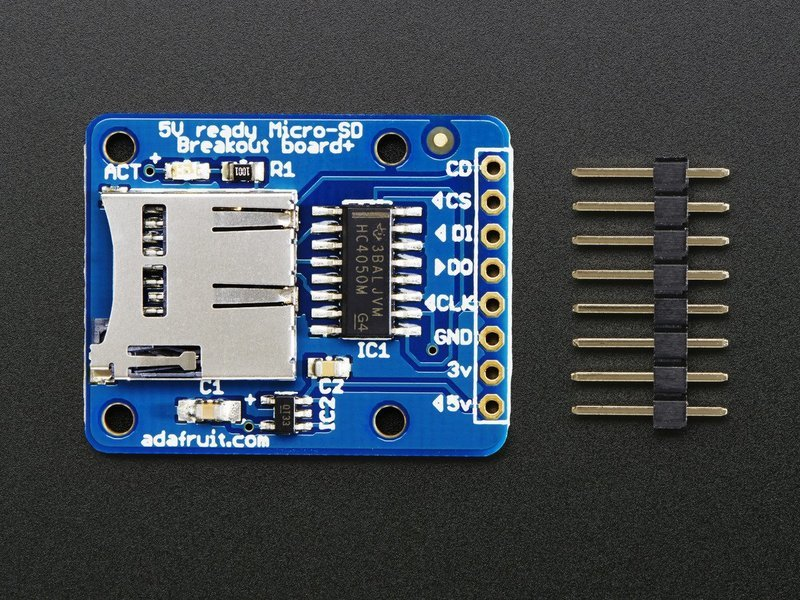
\includegraphics[width=\textwidth]{graphics/prototyping/micro_sd_card_breakout.png} 
\captionof{figure}{$\mu$SD-Card Breakoutboard \cite{ladyada2018}}
\label{fig:mikroSDKarten_breakoutboard}
\end{minipage}}

Die Abbildungen \ref{fig:bme280_breakoutboard}, \ref{fig:ds3231_breakoutboard} und \ref{fig:mikroSDKarten_breakoutboard} zeigen die jeweiligen im Prototyp benötigten Breakoutboards. Wie alles miteinander verbunden wurde, wird auf das Schema im Anhang \ref{pdf:schema} verwiesen. Zudem wurde mit diesen Bauteilen ein erster PCB-Entwurf designed (Anhang \ref{pdf:pcb}), sowie auch davon ein 3D-Modell (Anhang \ref{pdf:3d_modellierung}). Da alle Bauteile mit 3.3V betrieben werden können, ist das gesamte System für eine Betriebsspannung von 3.3V designed worden.

\newpage


{\begin{minipage}[b][5cm][t]{0.55\textwidth}
Über die USB-Schnittstelle werden die von der Sensorik erfassten Messdaten ausgegeben. Mittels eines Emulators (z.B. Putty) kann der COM-Port ausgelesen und die Daten dargestellt werden.\\

Zuerst werden dafür die partiellen Systeme initialisiert und die erfolgreiche Initialisierung ausgegeben. Danach beginnt der Messvorgang, wobei den Daten noch der Zeitstempel zugewiesen wird. Dann erfolgt die Ausgabe der Sensordaten (siehe Abb. \ref{fig:datenausgabe}).\\
\end{minipage}}
{\begin{minipage}[b][5cm][t]{0.44\textwidth}
\centering
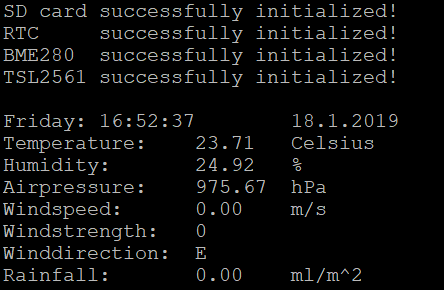
\includegraphics[width=\textwidth]{graphics/prototyping/ausgabe.PNG}
\captionof{figure}{Datenausgabe}
\label{fig:datenausgabe}
\end{minipage}}